\chapter{Vortex lattice}

El mètode de resolució emprat és el Vortex lattice. Aquest es basa en la teoria de lifting line de Prandtl, següents la qual la sustentació en una ala es pot plantejar com una sèrie de segments de vorticitat que generen unes velocitats induïdes als punts del seu voltant. Cal recalcar que aquesta teoria es troba dins del marc de fluid potencial, i per tant no té en compte efectes de viscositat.

Aquest mètode s'utilitza per resoldre l'aerodinàmica d'ales primes, ja que en els seus càlculs només té en compte els efectes de la curvatura i de l'angle d'atac, suposant que el perfil no té espessor. Es diferencia d'altres mètodes com el Lifting line perquè permet el càlcul d'ales de qualsevol aspect ratio.

Per tal de simplificar el plantejament del mètode de vortex lattice a continuació es descriu per la resolució d'una ala aïllada. En els següents apartats ja es descriuen les possibles modificacions que cal tenir en compte en afegir l'efecte terra o els efectes dels estabilitzadors vertical i horitzontal.

\section{Desenvolupament}

Com en la majoria de mètodes numèrics, cal discretitzar el domini a estudiar, en aquest cas l'ala. Es fan $N_{x}$ divisions en l'eix X i $N_{y}$ divisions en l'eix Y.

El següent pas és trobar la disposició dels anells de vorticitat. Aquest mètode planteja que en cada un dels panells que forma l'ala s'hi troba un anell de vorticitat, que genera una velocitat induïda a tots els punts de control de l'ala. Els anells es troben situats a $1/4$ de la corda de cada panell, tal i com es pot veure en verd a la figura \ref{discretit}.

\begin{figure}[h]
	\centering
	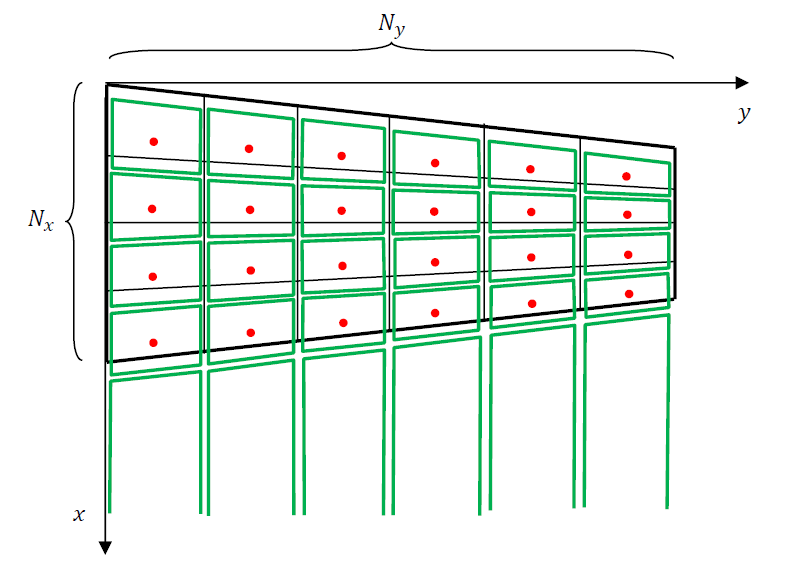
\includegraphics[scale=0.5]{./plots/discretitzacio}
	\caption{Discretització d'una semi-ala \cite{LizandraDalmases2017b}}
	\label{discretit}
\end{figure}

En la mateixa figura també es troben representats en color vermell els punts de control. Aquests són els punts on es calcula la velocitat induïda generada per tots els anells de vorticitat de l'ala. La velocitat induïda en un punt de control $i$ deguda a una anell de vorticitat $j$ és la suma de les velocitats induïdes per cada un dels segments que formen l'anell de vorticitat. És a dir:
\begin{equation}
\vec{v}_{ij}=\vec{v}_{ij_{AB}}+\vec{v}_{ij_{BC}}+\vec{v}_{ij_{CD}}+\vec{v}_{ij_{DA}}
\end{equation}
I la velocitat de cada segment ve determinada per l'expressió \cite{LizandraDalmases2017}:
\begin{equation}
\vec{v}_{ij_{segment}}=\frac{1}{4\pi}\frac{|\vec{r}_{1}|+|\vec{r}_{2}|}{|\vec{r}_{1}||\vec{r}_{2}|(|\vec{r}_{1}||\vec{r}_{2}|+\vec{r}_{1}\cdot\vec{r}_{2})}
\end{equation}
on $\vec{r}_{1}$ i $\vec{r}_{1}$ són les distàncies del punt de control als extrems del segment de vorticitat.

No obstant, en el càlcul de les velocitats induïdes pels anells de vorticitat cal tenir en compte que en el caire de sortida els anells de vorticitat en realitat són vòrtexs semi-infinits, com els que es veuen a la figura \ref{discretit}. En altres paraules, no són anells tancats, sinó que venen de l'infinit i se'n van a l'infinit. L'expressió de la velocitat induïda per un d'aquests segments semi-infinits és \cite{LizandraDalmases2017}:
\begin{equation}
\vec{v}_{ij_{segment}}=\frac{1}{4\pi}\frac{\vec{u}_{r}\times\vec{r}}{|\vec{u}_{r}\times\vec{r}|^{2}}
\end{equation}
on $u_{r}$ és el vector unitari que indica el sentit del segment i $r$ és la distancia entre el punt de control i el punt on comença o acaba el segment.

Per tant, la velocitat induïda final en cada punt de control serà la suma de les velocitat calculades per a cada vòrtex multiplicada pel seu valor de circulació. És a dir:
\begin{equation}
\vec{v}=\sum_{j=1}^{N}\Gamma_{j}\vec{v}_{ij}
\end{equation}

Un cop definides les velocitats de l'ala, cal plantejar el sistema d'equacions a resoldre per a obtenir la circulació de cada panell de l'ala i, en conseqüència, la sustentació. La condició que s'imposa és que la velocitat normal a l'ala en els punts de control sigui nul·la. Per a poder expressar aquesta condició cal afegir l'efecte de la velocitat aerodinàmica a les velocitats induïdes. És a dir, el sistema a resoldre és:
\begin{equation}
\left[\vec{U}_{\infty}+\sum_{j=1}^{N}\Gamma_{j}\vec{v}_{ij}\right]\cdot\vec{n}_{i}=\vec{U}_{\infty}\cdot\vec{n}_{i}+\sum_{j=1}^{N}\Gamma_{j}\left[\vec{v}_{ij}\cdot\vec{n}_{i}\right]=0
\end{equation}
on $\vec{U}_{\infty}$ és la velocitat aerodinàmica i $\vec{n}_{i}$ és el vector normal al perfil en el punt de control.

Per tal de simplificar aquest sistema, aquest es pot expressar de la següent forma:
\begin{equation}
\sum_{j=1}^{N}a_{ij}\Gamma{j}=b_{i}
\end{equation}
on $a_{ij}$ són els coeficients d'influència:
\begin{equation}
a_{ij}=\vec{v}_{ij}\cdot\vec{n}_{i}
\end{equation}
i $b_{i}$ és el terme de la dreta (RHS):
\begin{equation}
b_{i}=-\vec{U}_{\infty}\cdot\vec{n}_{i}
\end{equation}

Finalment, un cop obtingut el valor de la circulació, es pot procedir al càlcul de les forces i moments aerodinàmics. Començant per la sustentació:
\begin{equation}
L=\sum_{j=1}^{N_{y}}\sum_{i=1}^{N_{x}}\Delta L_{ij}=\rho U_{\infty}\sum_{j=1}^{N_{y}}\left[\Gamma_{1,j}+\sum_{i=2}^{N_{x}}\left(\Gamma_{i,j}-\Gamma_{i-1,j}\right)\right]\Delta y_{i}
\end{equation}
\begin{equation}
C_{L}=\frac{L}{\frac{1}{2}\rho U_{\infty}^{2}S}
\end{equation}
on $U_{\infty}$ és el mòdul de la velocitat aerodinàmica, $\rho=1,225 kg/m^{3}$ la densitat de l'aire i $S$ la superfície alar.

El càlcul de la resistència aerodinàmica és més complicat, ja que aquesta consta de dos termes: resistència paràsita i resistència induïda.

DRAG I MOMENT!!!!

\section{Algoritme}
\label{algoritmeala}
L'algoritme utilitzat per a resoldre el plantejament proposat es troba esquematitzat a continuació.

\begin{figure}[H]
	\centering
	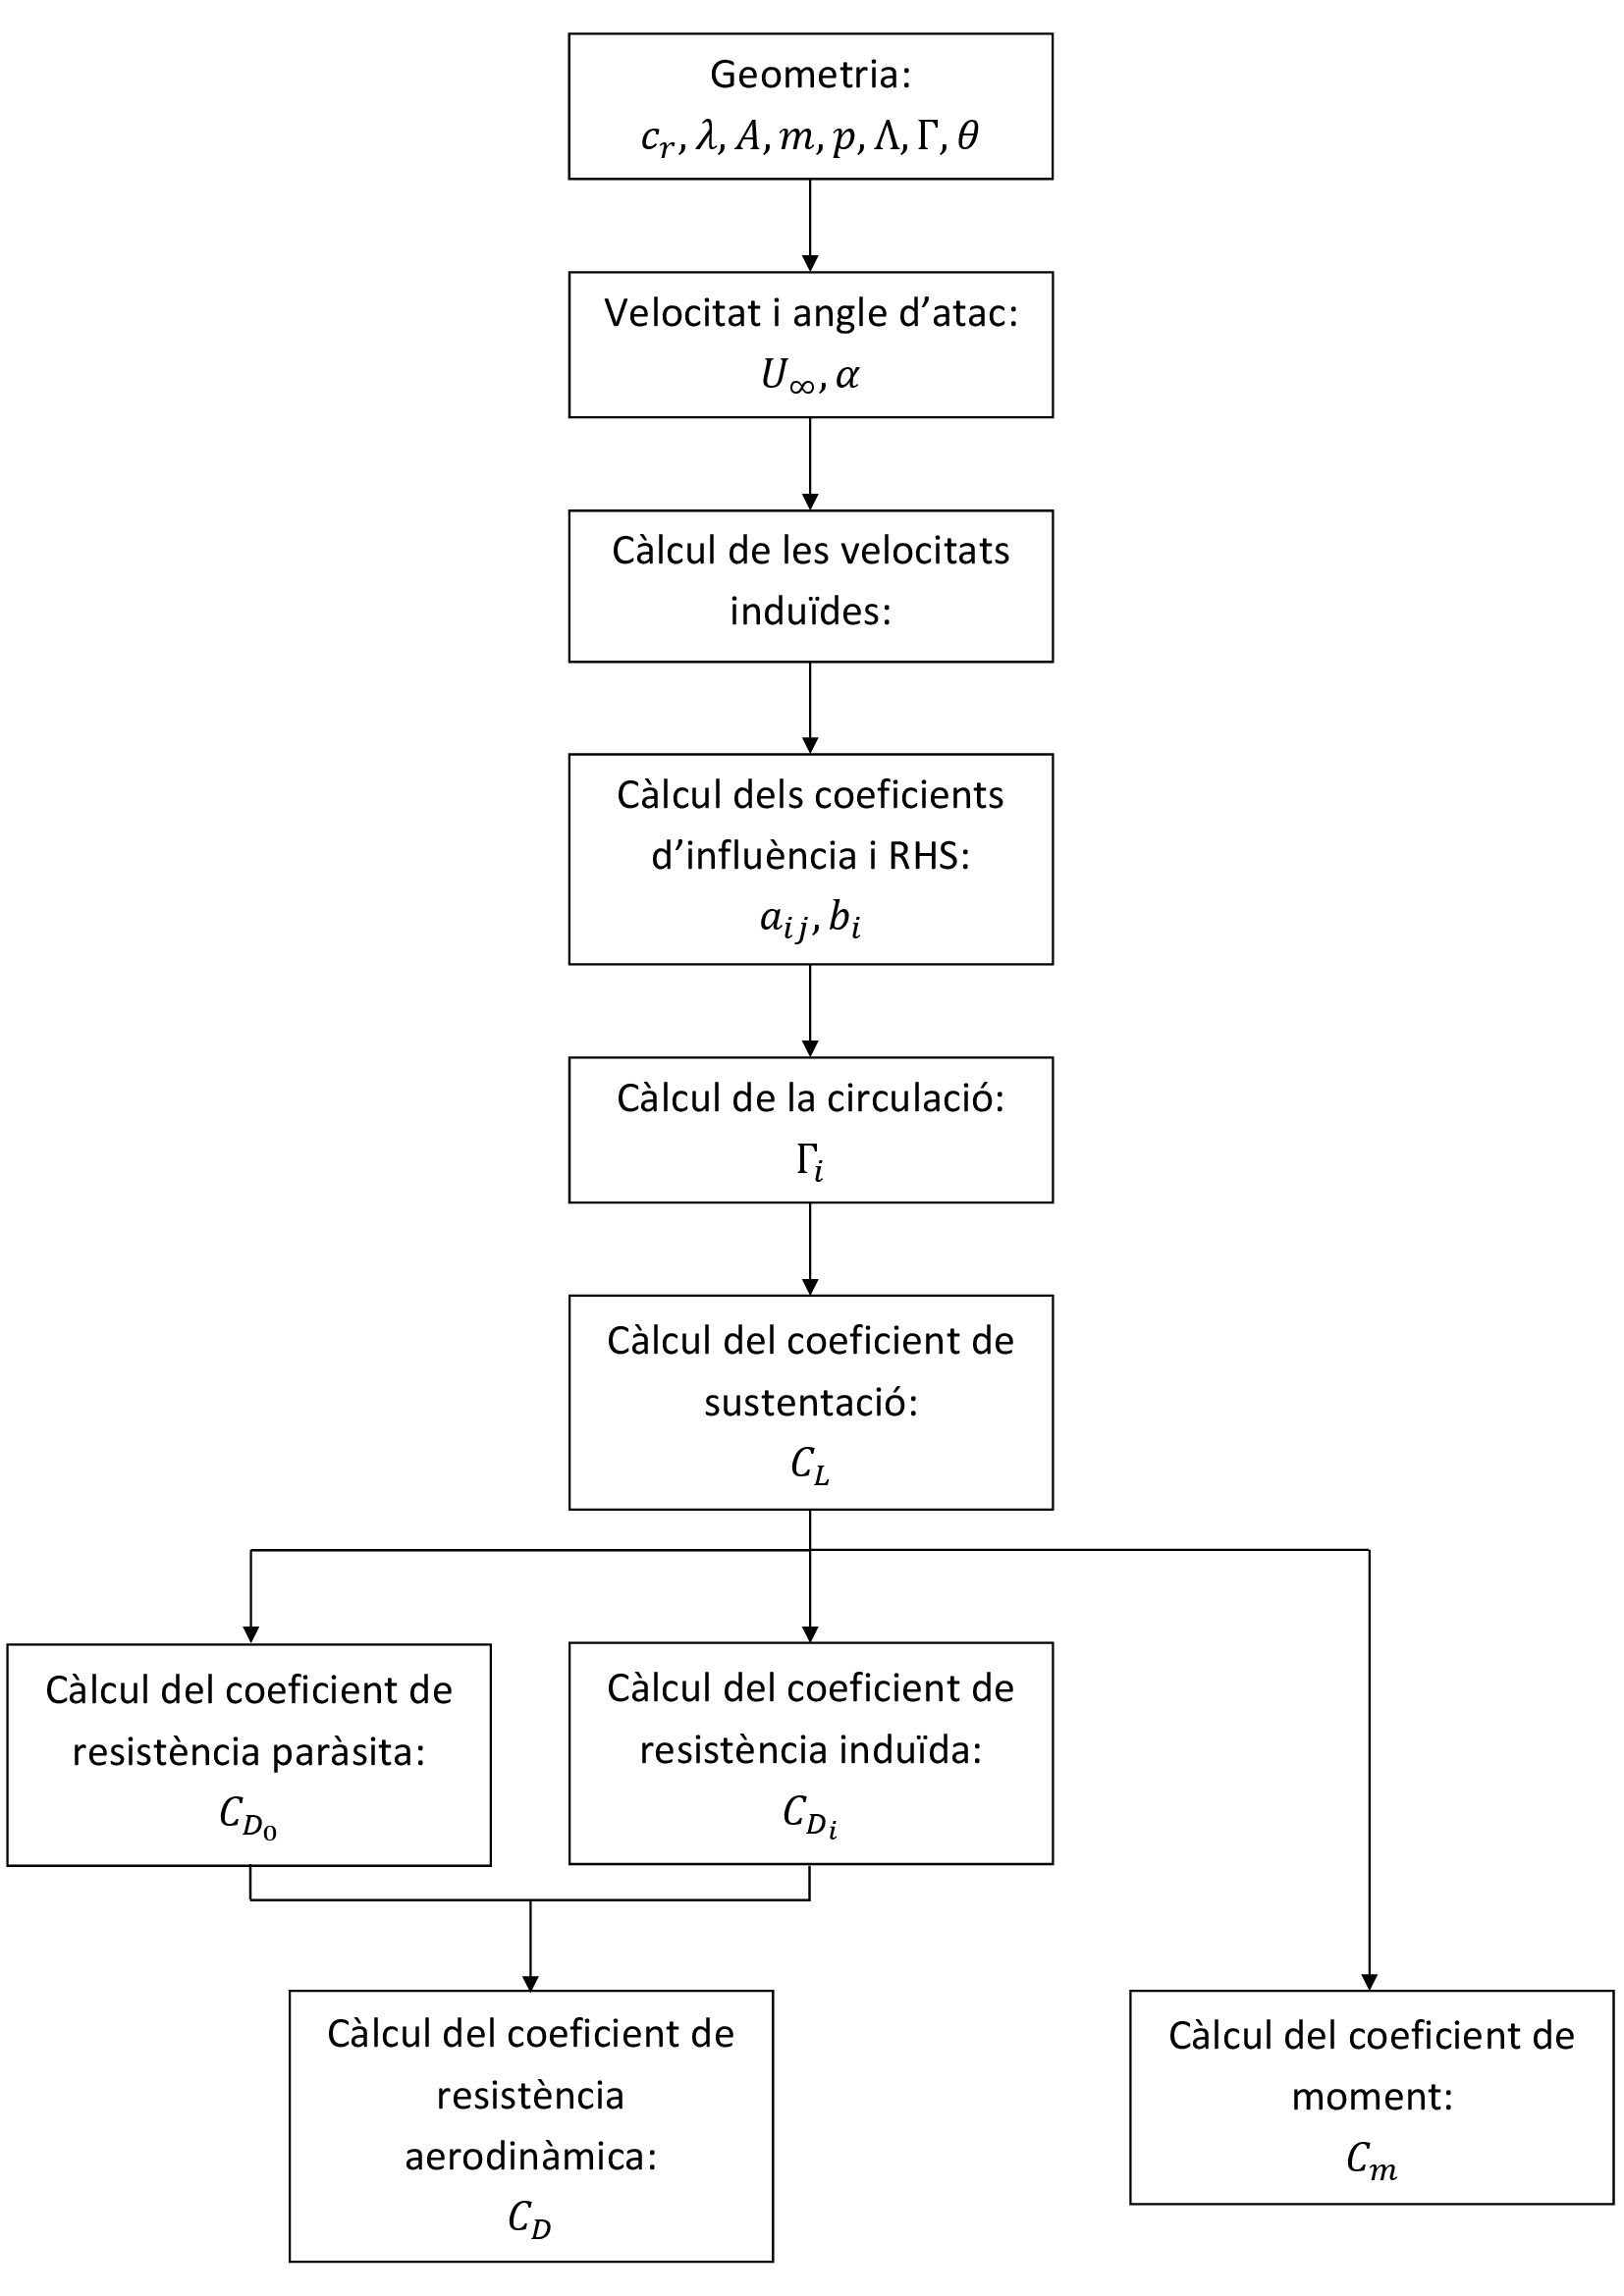
\includegraphics[scale=0.185]{./plots/algoritmewing}
\end{figure}